\RussianSourceFrame{GELFAND-P001405}{unlabelled}
Тогда
\begin{equation*}
(Y_I,Y_J)=\text{\RussianUnclear{GELFAND-P001405}{pairing-value}{0 или C}}
\quad\text{при }J\ne I'.\tag{35}
\end{equation*}
(всё в факторах)

\underline{Теорема:}

(36) $Z[x_1,x_2,x_3]$ — своб. модуль [вставлено над строкой: над]
$\underline{\operatorname{Sym}}(x_1,x_2,x_3)$
с базисом — полин. Шуберта.

Не все полин. Шуберта явл. детерминантами и поэтому вместо
них используются разд. разности $\partial_i$.

\underline{Зад. И.М.Г.} Обобщить теор. о характерах: непр. предст., характеры
\RussianUnclear{GELFAND-P001405}{characters-line-ending}{с-…-}
-ф-и Шуберта.

\underline{След. раз будет Тахтаджян о квантовых группах.}

\underline{\underline{Капранов (Миша)}}

\underline{2-категории.}

Это алг. структ. с объектами 4-х типов
\begin{description}
\item[а)] объекты $\bullet$
\item[б)] гориз. морф. $\bullet\longrightarrow\bullet$
\item[в)] верт. морф. $\uparrow$
\item[г)] квадраты
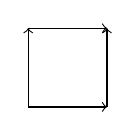
\begin{tikzpicture}[baseline=0.3cm]
\draw[->] (0,0)--(1,0);
\draw[->] (0,1)--(1,1);
\draw[->] (0,0)--(0,1);
\draw[->] (1,0)--(1,1);
\end{tikzpicture}
\end{description}

[На правом поле:]
Здесь $\begin{matrix}\longrightarrow\\\longrightarrow\end{matrix}$ гориз. морф.,
$\uparrow\ \uparrow$ верт. морф.
(их нач. и концы — 1-морфизмы).

Можно компонировать:
\begin{description}
\item[1)] $\longrightarrow\ \longrightarrow$ 2 гориз. морф.
\item[2)] $\begin{matrix}\uparrow\\\uparrow\end{matrix}$ 2 верт. морф.
\item[3)] квадр. двумя способами умножаются
\end{description}
\begin{center}
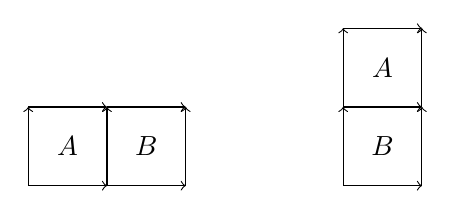
\begin{tikzpicture}
\draw[->] (0,0)--(1,0);
\draw[->] (1,0)--(2,0);
\draw[->] (0,1)--(1,1);
\draw[->] (1,1)--(2,1);
\draw[->] (0,0)--(0,1);
\draw[->] (1,0)--(1,1);
\draw[->] (2,0)--(2,1);
\node at (0.5,0.5) {$A$};
\node at (1.5,0.5) {$B$};
\draw[->] (4,0)--(5,0);
\draw[->] (4,1)--(5,1);
\draw[->] (4,2)--(5,2);
\draw[->] (4,0)--(4,1);
\draw[->] (4,1)--(4,2);
\draw[->] (5,0)--(5,1);
\draw[->] (5,1)--(5,2);
\node at (4.5,1.5) {$A$};
\node at (4.5,0.5) {$B$};
\end{tikzpicture}
\end{center}
(см. книгу Габриэля)
% Review coordinates (original pixels): pairing [720,125,890,280];
% characters ending [1980,1020,2360,1120]; full-page 2408 x 3448.


\RussianSourceFrame{GELFAND-P001406}{33}
\underline{Осн. нетрив. аксиома}: 2-мерн. ассоциативность

(1)
\RussianSourceFigure{GELFAND-P001406}{interchange-diagram}{Слева два вертикальных прямоугольника: в первом $A$ над $B$, во втором $C$ над густо обведённым знаком, похожим на $D$; в каждом средняя горизонтальная стрелка направлена вправо. Между прямоугольниками кружок композиции, далее знак равенства. Справа верхний ряд содержит $A$, $C$, нижний — $B$, знак, похожий на $D$; между рядами узкая полоса с кружком. У концов полосы видны стрелочные и повторно обведённые штрихи, точное соединение которых неясно.}

\begin{center}
\begin{minipage}[t]{.46\linewidth}\vspace{0pt}\centering
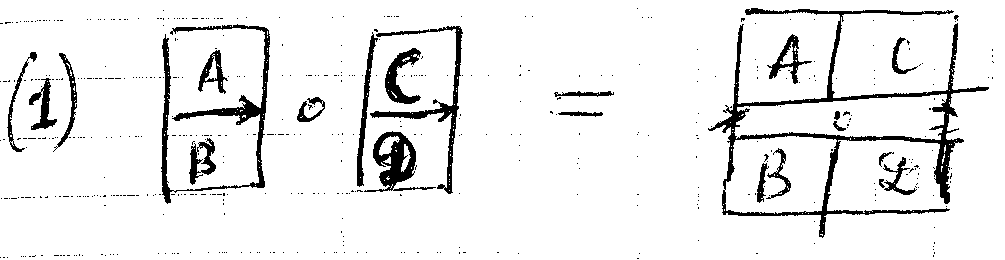
\includegraphics[width=\linewidth]{figures/gelfand-0153-p001406-interchange-original.png}\par\smallskip
{\footnotesize Оригинал рукописного рисунка: \texttt{GELFAND-P001406}}
\end{minipage}\hfill
\begin{minipage}[t]{.50\linewidth}\vspace{0pt}\centering
{\footnotesize Частичное воссоздание видимых штрихов}\par\smallskip
\resizebox{\linewidth}{!}{% Visible-stroke transcription; D? and the retraced side connections remain unresolved.
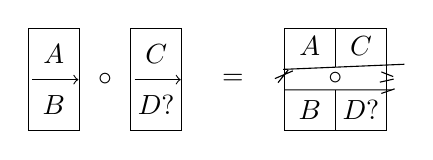
\begin{tikzpicture}[x=.65cm,y=.65cm]
\draw (0,0) rectangle (1,2); \draw[->] (.08,1)--(.98,1);
\node at (.5,1.5) {$A$};\node at (.5,.5) {$B$};
\node at (1.5,1) {$\circ$};
\draw (2,0) rectangle (3,2);\draw[->] (2.08,1)--(2.98,1);
\node at (2.5,1.5) {$C$};\node at (2.5,.5) {$D?$};
\node at (4,1) {$=$};
\draw (5,0)--(7,0)--(7,2)--(5,2)--cycle;
\draw (5,.8)--(7.1,.8) (4.98,1.2)--(7.35,1.3);
\draw (6,0)--(6,.8) (6,1.25)--(6,2);
\node at (5.5,1.65) {$A$};\node at (6.5,1.65) {$C$};
\node at (5.5,.4) {$B$};\node at (6.5,.4) {$D?$};
\node at (6,1.02) {$\circ$};
% Plain crossing strokes preserve uncertainty and do not declare arrows.
\draw (4.82,1.02)--(5.17,1.17) (4.88,.94)--(5.08,1.19);
\draw (6.9,1.15)--(7.13,1.06) (6.87,.95)--(7.14,1.01)
 (6.9,.73)--(7.16,.82);
\end{tikzpicture}
}
\end{minipage}
\end{center}
\noindent{\small\textit{Две подписи, похожие на D, и обведённые боковые штрихи не установлены. Боковые линии не утверждают направления стрелок.}}


\underline{Пример, когда не вып.}
[зачёркнуто: \RussianUnclear{GELFAND-P001406}{example-cancel-left}{неразборчиво}]
акс.
[зачёркнуто: \RussianUnclear{GELFAND-P001406}{example-cancel-right}{неразборчиво}]
(1)

\underline{Тензоры:}
\begin{center}
\begin{tikzpicture}
\draw (0,0)--(1,0)--(1,1)--(0,1)--cycle;
\node at (0.5,0.5) {$A$};
\node at (-0.25,1.15) {$k$};
\node at (1.25,1.15) {$\ell$};
\node at (-0.25,-0.25) {$i$};
\node at (1.25,-0.25) {$j$};
\draw (2,0)--(3,0)--(3,1)--(2,1)--cycle;
\node at (2.5,0.5) {$B$};
\node at (1.75,1.25) {$\ell$};
\node at (3.25,1.15) {$r$};
\node at (1.75,-0.25) {$j$};
\node at (3.25,-0.05) {$s$};
\node at (5,0.5) {свёртка};
\end{tikzpicture}
\end{center}
\begin{equation*}
(AB)_{ik}^{rs}=\sum A_{ij}^{k\ell}B_{js}^{\ell r}
\end{equation*}
\RussianUnclear{GELFAND-P001406}{tensor-indices}{Положение индексов сохранено по рукописи.}

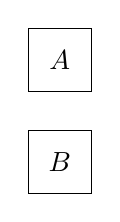
\begin{tikzpicture}
\draw (0,1.3)--(0.8,1.3)--(0.8,2.1)--(0,2.1)--cycle;
\node at (0.4,1.7) {$A$};
\draw (0,0)--(0.8,0)--(0.8,0.8)--(0,0.8)--cycle;
\node at (0.4,0.4) {$B$};
\end{tikzpicture}

Аксиома (1) не будет выполнена.

\underline{Другое опр.} (М. Концевич) (конкурирующее)

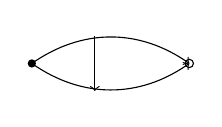
\begin{tikzpicture}[baseline=0cm]
\fill (0,0) circle (1.5pt);
\draw (2,0) circle (1.5pt);
\draw[->] (0,0) to[bend left=35] (2,0);
\draw[->] (0,0) to[bend right=35] (2,0);
\draw[->] (0.8,0.35)--(0.8,-0.35);
\end{tikzpicture}
морфизмы между морф. с одинаков. концами.

\underline{Пример:} $Cat$ (категория категорий; есть морфизм
функторов)

Это частный случай предыдущего (стягиваем верт. стрелки)

\underline{И.М.Г.}

\RussianSourceFigure{GELFAND-P001406}{boundary-diagram}{В квадрате написано $\Delta u=0$. У верхней и нижней сторон горизонтальные стрелки направлены вправо; у левой стороны две внутренние вертикальные стрелки направлены вверх. Слева подписано $u$ и $\frac{\partial u}{\partial n}$; над этой подписью ещё одно неясное обозначение.}

\begin{center}
\begin{minipage}[t]{.46\linewidth}\vspace{0pt}\centering
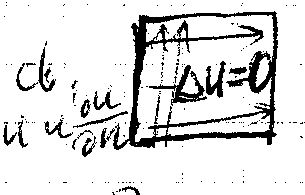
\includegraphics[width=\linewidth]{figures/gelfand-0153-p001406-boundary-original.png}\par\smallskip
{\footnotesize Оригинал рукописного рисунка: \texttt{GELFAND-P001406}}
\end{minipage}\hfill
\begin{minipage}[t]{.50\linewidth}\vspace{0pt}\centering
{\footnotesize Частичное воссоздание видимых штрихов}\par\smallskip
\resizebox{\linewidth}{!}{\begin{tikzpicture}[x=1.2cm,y=1.2cm]
\draw (0,0) rectangle (1.1,1);
\draw[->] (.05,.83)--(1.04,.83);\draw[->] (.03,.13)--(1.06,.19);
\draw[->] (.15,.1)--(.19,.95);\draw[->] (.29,.13)--(.36,.96);
\node at (.69,.55) {$\Delta u=0$};
\node[left] at (-.05,.6) {$[?]$};
\node[left] at (-.06,.05) {$u,\ \dfrac{\partial u}{\partial n}$};
\end{tikzpicture}
}
\end{minipage}
\end{center}
\noindent{\small\textit{Верхнее левое обозначение остаётся [?] после просмотра при 3×, 5× и 10×. Видимые u и нормальная производная набраны; граничное условие не дополнено.}}

гран. условия

Просьба к Келдышу — Ченцову — Гельфанду

\underline{К.} Высшие фунд. гр.
$X_0\subset X_1\subset X$ — топ. пр-во

объекты — точки $x\in X_0$

морф.
$\bigl(\underset{\text{отрезок}}{I},\partial I\bigr)\longrightarrow(X_1,X_0)$
\qquad гомотопные $(\mathrm{mod}\ \partial I)$ счит. эквив.

биморфизмы
$(I^2,\partial I^2)\longrightarrow(X,X_1)$
\qquad $(\mathrm{mod}\ \text{\underline{гомотопии}})$
% Review coordinates (original pixels): label [2220,20,2370,180];
% indices [390,950,1230,1160]; boundary diagram [245,2260,550,2455];
% cancelled groups [970,465,1050,530] and [1165,460,1300,565].


\RussianSourceFrame{GELFAND-P001407}{44}
\underline{\underline{23/XI-87 г.}} \qquad \underline{Сем. Гельфанда.}

\underline{Бейлинсон} (продолжение)

\underline{Производные категории.}

(1) \underline{Лемма:}
\begin{equation*}
\begin{tikzcd}[column sep=small,row sep=small]
X^\bullet && Y^\bullet\\
& Z^\bullet \arrow[ul,"{\text{квази-изом.}}"] \arrow[ur] &
\end{tikzcd}
\quad\Rightarrow\quad\exists\quad
\begin{tikzcd}[column sep=small,row sep=small]
& Z'^\bullet &\\
X^\bullet \arrow[ur,"{\text{квазиизом}}"] && Y^\bullet \arrow[ul]
\end{tikzcd}
\end{equation*}

Лемма док. с пом. конструкции конуса отображения.

\underline{Напоминание:}

$\mathcal{A}$ — аб. категория
\begin{equation*}
\begin{array}{ccccc}
C(\mathcal{A}) & \longrightarrow & K(\mathcal{A}) & \longrightarrow & D(\mathcal{A})\\
\text{комплексы} && \substack{\text{гомотоп.}\\\text{катег.}\\\text{комплексов}} &&
\substack{\text{производная}\\\text{категория}}
\end{array}
\end{equation*}
[Справа:] (объекты всюду суть комплексы)

$f:X^\bullet\to Y^\bullet$ гомотопно $0$, если
$\exists g^i:X^i\to Y^{i-1}$,
\begin{equation*}
f^i=dg^i+g^{i+1}d
\end{equation*}

$D(\mathcal{A})$ — это $K(\mathcal{A})$ с обращенными
\underline{квазиизоморфизмами}
(морф., индуц. изоморфизм когомологий)

Морфизм из $X^\bullet$ в $Y^\bullet$ — это диаграмма в $K(\mathcal{A})$
\begin{equation*}
\begin{tikzcd}[column sep=small,row sep=small]
X^\bullet && Y^\bullet\\
& Z^\bullet \arrow[ul,"\sim"] \arrow[ur] &
\end{tikzcd}
\tag{2}
\end{equation*}
(левая стрелка — квазиизоморфизм)

точнее, класс эквивал. таких диаграмм: диагр. (2) эквивалентна
диаграмме, полученной с пом. любого квазиизоморфизма
$\chi:Z'^\bullet\to Z^\bullet$
\begin{equation*}
\begin{tikzcd}[column sep=small,row sep=small]
X^\bullet && Y^\bullet\\
& Z^\bullet \arrow[ul,"\varphi"',"\sim"] \arrow[ur,"\psi"] &\\
& Z'^\bullet \arrow[u,"\chi"',"\sim"] &
\end{tikzcd}
\qquad
\begin{tikzcd}[column sep=small,row sep=small]
X^\bullet && Y^\bullet\\
& Z' \arrow[ul,"{\varphi\circ\chi}"',"\sim"] \arrow[ur,"{\psi\circ\chi}"'] &
\end{tikzcd}
\tag{3}
\end{equation*}

(это отношение продолжается до наименьшего содержащего его
отношения эквивалентности)

Конус морфизма и точные треугольники были определены
[зачёркнуто: \RussianUnclear{GELFAND-P001407}{last-line-cancellation}{неразборчиво}]
ещё.
% Review coordinates (original pixels): (1) [150,375,1370,735];
% (2) [290,1900,800,2200]; (3) [210,2320,1640,2760];
% final cancellation [1970,2925,2085,2990], inspected at 10x.
% Composition circles confirmed at 10x: [1195,2415,1335,2540] and
% [1450,2440,1610,2570].


\RussianSourceFrame{GELFAND-P001408}{unlabelled}
% Original image: 2408 x 3448 pixels. Coordinates below use the original pixel grid.
% Header and first example: (250,65)-(2150,745).
\underline{И. Захаревич}
[зачёркнуто: \RussianUnclear{GELFAND-P001408}{cancelled-title}{неразборчиво}]
\underline{Импровизация \RussianUnclear{GELFAND-P001408}{title-preposition}{о / с} хаосе.}

\underline{Примеры}

$1^{\circ}$. Видимо, есть морфизм из одного примера в другой.
\begin{equation*}
M=(\mathbb{Z}/2\mathbb{Z})^{\mathbb{Z}}
\qquad\text{(беск. в обе стороны послед.)}
\end{equation*}
$T\colon M\to M$. На $M$ станд. топология (кантор. мн-во).
\begin{equation*}
a_i\to a_{i-1}\qquad\text{(преобр. сдвига; преобр. Бернулли)}
\end{equation*}
Рассм. итерации: $T^N$.

% Baker transformation and cancellations: (300,725)-(2250,1590).
На $M$ есть мера. Преобр. пекаря совпадает с этим
[вставлено над строкой: (с точн. до меры $0$)]
[зачёркнуто после «этим» и строкой ниже:
\RussianUnclear{GELFAND-P001408}{baker-cancellations}{неразборчиво}].

% Confidently visible labelled axes and folding arrow: (390,950)-(940,1285).
\begin{center}
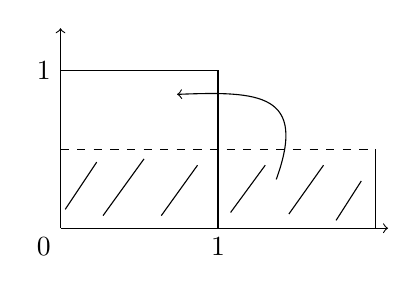
\begin{tikzpicture}[x=2cm,y=2cm]
\draw[->] (0,0) -- (2.08,0);
\draw[->] (0,0) -- (0,1.27);
\draw (0,1) -- (1,1) -- (1,0);
\draw (2,0) -- (2,0.5);
\draw[dashed] (0,0.5) -- (2,0.5);
\draw (0.03,0.12) -- (0.23,0.42);
\draw (0.27,0.08) -- (0.53,0.44);
\draw (0.64,0.08) -- (0.87,0.4);
\draw (1.08,0.1) -- (1.3,0.4);
\draw (1.45,0.09) -- (1.67,0.4);
\draw (1.75,0.05) -- (1.91,0.3);
\draw[->] (1.37,0.31) .. controls (1.57,0.86) and (1.26,0.87) .. (0.74,0.85);
\node[below left] at (0,0) {$0$};
\node[left] at (0,1) {$1$};
\node[below] at (1,0) {$1$};
\end{tikzpicture}
\end{center}

\RussianSourceFigure{GELFAND-P001408}{baker-sequence}{Три рисунка слева направо: квадрат с замкнутой округлой кривой и горизонтальной пунктирной линией; квадрат с двумя вытянутыми изгибами, входящими с противоположных сторон; квадрат с несколькими почти горизонтальными полосами и короткими петлеобразными изгибами у краёв. В третьем рисунке различима стрелка влево на нижней длинной линии; направление мелких штрихов первого и третьего рисунков не вполне ясно.}

\begin{center}
\begin{minipage}[t]{.46\linewidth}\vspace{0pt}\centering
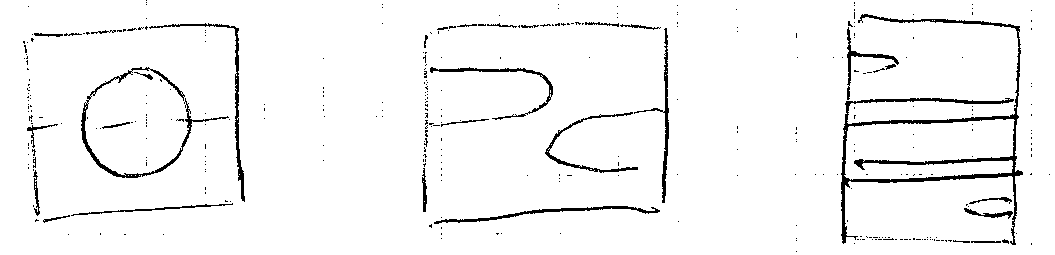
\includegraphics[width=\linewidth]{figures/gelfand-0153-p001408-baker-sequence-original.png}\par\smallskip
{\footnotesize Оригинал рукописного рисунка: \texttt{GELFAND-P001408}}
\end{minipage}\hfill
\begin{minipage}[t]{.50\linewidth}\vspace{0pt}\centering
{\footnotesize Частичное воссоздание видимых штрихов}\par\smallskip
\resizebox{\linewidth}{!}{% Only the clear leftward long arrow is interpreted as a direction.
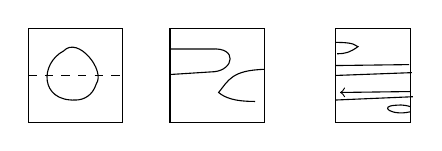
\begin{tikzpicture}[x=.6cm,y=.6cm]
\draw (0,0) rectangle (2,2);\draw[dashed] (0,1)--(2,1);
\draw (1,.48) .. controls (.25,.45) and (.24,1.25) .. (.75,1.52)
 .. controls (1.05,1.84) and (1.64,1.11) .. (1.44,.82)
 .. controls (1.36,.57) and (1.17,.48) .. (1,.48);
\draw (3,0) rectangle (5,2);
\draw (3,1.56)--(3.88,1.56) .. controls (4.44,1.6) and (4.35,1.12) .. (3.94,1.08)--(3,1.02);
\draw (5,1.13) .. controls (4.31,1.11) and (4.24,.9) .. (4.03,.64)
 .. controls (4.16,.53) and (4.36,.45) .. (4.8,.45);
\draw (6.5,0) rectangle (8.1,2);
\draw (6.5,1.7) .. controls (6.93,1.7) and (6.9,1.64) .. (6.98,1.61)
 .. controls (6.81,1.49) and (6.72,1.46) .. (6.54,1.46);
\draw (6.5,1.21)--(8.06,1.23) (6.5,1.0)--(8.12,1.06);
\draw[->] (8.1,.66)--(6.6,.64);\draw (6.5,.48)--(8.14,.55);
\draw (8.08,.23) .. controls (7.7,.14) and (7.4,.35) .. (7.78,.37)
 .. controls (7.93,.39) and (8.07,.35) .. (8.08,.34);
\end{tikzpicture}
}
\end{minipage}
\end{center}
\noindent{\small\textit{Видимые изгибы сохранены. Направление указано лишь у ясно различимой длинной стрелки влево; мелкие конечные штрихи не истолкованы.}}

и т. д.

% Binary correspondence and forward/backward iterates: (295,1590)-(2230,2260).
\underline{Соответствие}: записать коорд. точки квадрата в двоичной системе
и взять $1$ цифру — налево, другую — направо.

В каком смысле это хаос

Рассм. $T^k x$, $k\leq 0$ — пусть это известно (с точн. до $1$ мм).
\begin{equation*}
T^k x,\qquad k>0
\end{equation*}
за конечное время вся эта информ. потеряется.

% Second example: (305,2290)-(2400,2700).
$2^{\circ}$. \underline{Гиперболич. преобразование}:
геодезич. потоки на \RussianUnclear{GELFAND-P001408}{manifold-abbreviation}{мн-зиях / мн-иях} отриц. кривизны.

\RussianSourceFigure{GELFAND-P001408}{hyperbolic-surface}{Замкнутый контур с двумя расширениями и перетяжкой между ними. Внутри слева и справа нарисованы дуги, похожие на обозначения двух ручек поверхности; в средней части короткий наклонный отрезок с выделенными концами и ответвляющейся стрелкой вправо-вверх. Мелкие направления и точное соединение внутренних дуг требуют проверки оригинала.}

\begin{center}
\begin{minipage}[t]{.46\linewidth}\vspace{0pt}\centering
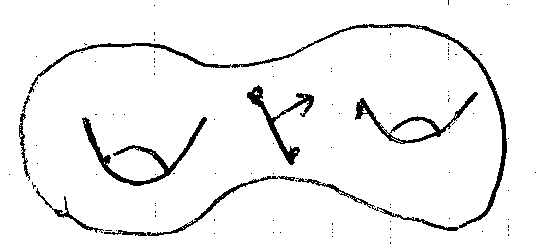
\includegraphics[width=\linewidth]{figures/gelfand-0153-p001408-hyperbolic-surface-original.png}\par\smallskip
{\footnotesize Оригинал рукописного рисунка: \texttt{GELFAND-P001408}}
\end{minipage}\hfill
\begin{minipage}[t]{.50\linewidth}\vspace{0pt}\centering
{\footnotesize Частичное воссоздание видимых штрихов}\par\smallskip
\resizebox{\linewidth}{!}{% The drawn contour and interior arcs are reproduced without a genus assertion.
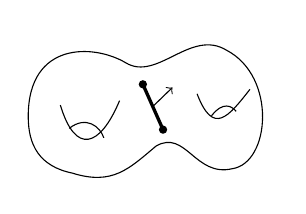
\begin{tikzpicture}[x=.8cm,y=.8cm]
\draw (0,1) .. controls (0,2.2) and (1.05,2.15) .. (1.55,1.85)
 .. controls (2.05,1.55) and (2.58,2.4) .. (3.15,2.05)
 .. controls (3.95,1.63) and (3.84,.26) .. (3.24,.17)
 .. controls (2.65,.03) and (2.5,.8) .. (2.03,.53)
 .. controls (1.6,.17) and (1.34,-.1) .. (.7,.1)
 .. controls (.17,.21) and (0,.55) .. (0,1);
\draw (.51,1.18) .. controls (.75,.38) and (1.14,.51) .. (1.45,1.25);
\draw (.65,.81) .. controls (.92,1.02) and (1.14,.84) .. (1.2,.66);
\draw (2.68,1.36) .. controls (2.94,.68) and (3.18,1.0) .. (3.52,1.43);
\draw (2.91,1.01) .. controls (3.09,1.24) and (3.23,1.17) .. (3.3,1.08);
\draw[very thick] (1.82,1.51)--(2.14,.79);
\fill (1.82,1.51) circle (1.5pt);\fill (2.14,.79) circle (1.5pt);
\draw[->] (1.97,1.15)--(2.29,1.46);
\end{tikzpicture}
}
\end{minipage}
\end{center}
\noindent{\small\textit{Воссозданы внешний контур, внутренние дуги, отмеченный отрезок и ответвляющаяся стрелка. Топология и метрика по эскизу не восстановлены.}}



\RussianSourceFrame{GELFAND-P001409}{45}
% Original image: 2408 x 3448 pixels. All coordinates refer to original pixels.
% Header: (205,35)-(2280,200).
\underline{Г. Маргулис.}
\underline{Итерации отображений компл. плоскости.}

Рассм. преобр. $z\to P(z)$, $P$ — многочлен

(более общо — рац. ф-я)

$\operatorname{deg}P=1$
[зачёркнуто: \RussianUnclear{GELFAND-P001409}{degree-one-cancellation}{неразборчиво}]
неинтересный случай

$(1)\quad z\mapsto az+b$

\underline{Итерации}:
\begin{equation*}
z_{i+1}=P(z_i)
\end{equation*}
$|a|>1\Rightarrow$ одна неподв. точка;

\RussianUnclear{GELFAND-P001409}{unit-modulus-claim}{$|a|=1\Rightarrow$ всё разбив. на инвар. окружности, на к-рых поворот.}

% Three nested circular contours with a central point: (265,985)-(580,1235).
\begin{center}
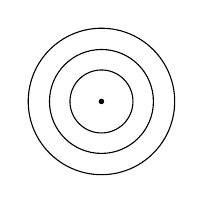
\begin{tikzpicture}
\draw (0,0) circle (0.4);
\draw (0,0) circle (0.66);
\draw (0,0) circle (0.93);
\fill (0,0) circle (0.035);
\end{tikzpicture}
\end{center}

% Gelfand interjection: (135,1240)-(2340,1745).
\underline{И. М. Г.}: 1) вопрос о том, когда преобраз. окружности диффеоморфно повороту,
нетривиален: Данжуа, Арнольд, Herman

2) Что такое представление дискретной бескон. группы?

Нет удовлетв. ответа.

Фон Неймановская теор. не эстетична.

На окружности возникает хаос.

\underline{Гипотеза}: если работать с мн-вами промежуточной хаусдорфовой
размерности, то нек-рая классика восстановится!!

% Covering question and tasks: (100,2070)-(2340,2820).
\underline{Вопрос для школьников}: покрываем $n$-е рац. число интервалом
длины $\varepsilon/2^n$. Привести пример числа, к-рое не будет покрыто.

\underline{Задача}: найти хаусд. размерность канторовского соверш. мн-ва.

\tikz\node[draw,circle,inner sep=2pt] {!};
\underline{Задача}. \underline{Построить теорию предст. дискр. групп на ф-ях на}
\underline{мн-вах промежут. хаусд. размерности.}

Для начала посмотреть физику — теор. струн и т. д.

% Margulis resumes: (170,2800)-(2180,3230).
\underline{Г. М.}:
$z\to z^2$
\qquad $|z|=1$ перех. в себя

\begin{center}
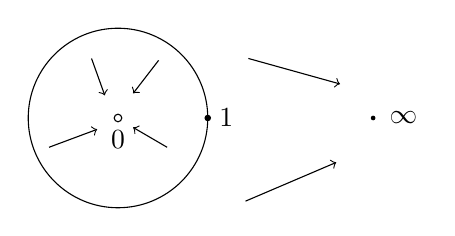
\begin{tikzpicture}[x=1.2cm,y=1.2cm]
\draw (0,0) circle (0.95);
\draw (0,0) circle (0.04);
\node[below] at (0,-0.03) {$0$};
\fill (0.95,0) circle (0.035);
\node[right] at (0.97,0) {$1$};
\draw[->] (-0.28,0.63) -- (-0.14,0.24);
\draw[->] (0.43,0.61) -- (0.16,0.26);
\draw[->] (0.52,-0.31) -- (0.16,-0.1);
\draw[->] (-0.73,-0.31) -- (-0.22,-0.12);
\draw[->] (1.38,0.63) -- (2.35,0.36);
\draw[->] (1.35,-0.88) -- (2.31,-0.47);
\fill (2.7,0) circle (0.025);
\node[right] at (2.77,0) {$\infty$};
\end{tikzpicture}
\end{center}
на окр. — аналог преобр. пекаря
(одностороннего)


\RussianSourceFrame{GELFAND-P001410}{unlabelled}
% Original image: 2408 x 3448 pixels. Coordinates use the original pixel grid.
% Iteration and normality definition: (140,40)-(2360,900).
\begin{equation*}
f_n=\underbrace{f\circ f\circ\cdots\circ f}_{n\ \text{раз}}
\end{equation*}
\underline{Опр.}

$U$ — [зачёркнуто: мн-во; над строкой вставлено: окр.]
нормальности; если $\left.f_n\right|_U$ — компактное мн-во

(норм. сем-во анал. ф-й)

[На отдельной короткой строке зачёркнуто:
\RussianUnclear{GELFAND-P001410}{isolated-cancellation}{неразборчиво}.]

Мн-во норм. [вставлено над строкой: $X$] сост. из точек $x$, для к-рых
$\exists$ окр. $U$ — [зачёркнуто:
\RussianUnclear{GELFAND-P001410}{normality-cancellation}{неразборчиво}]
окр. нормальности

[Под «Мн-во норм.»: (оно открыто)]

Дополнение к мн-ву нормальности — \underline{мн-во Жюлиа}.

(оно замкнуто)

Мн-во норм. может быть пусто

% Components and Sullivan's assertion: (160,900)-(2130,1790).
\begin{equation*}
X=X_1\cup\cdots\cup X_n\cup\cdots
\end{equation*}
(связные компоненты)

мн-ва нормальности

[зачёркнуто под этой подписью:
\RussianUnclear{GELFAND-P001410}{components-cancellation}{неразборчиво}]

\begin{equation*}
\begin{aligned}
f\colon (\text{св. компон.})&\to(\text{св. компоненты})\\
X_i&\mapsto X_{j(i)}
\end{aligned}
\end{equation*}
\underline{Sullivan} доказал, что в возникающем

[зачёркнуто: \RussianUnclear{GELFAND-P001410}{sullivan-cancellation}{неразборчиво}]
преобр. дискр. мн-ва (счётн. или конечного)

а) каждая орбита стабилизируется,

б) мн-во неподв. точек конечно.

\underline{Идея док-ва}. Пусть есть беск. орбита

% Five ovals with interior small circles; lower labels only 1,2,3,4: (335,1925)-(1195,2105).
\begin{center}
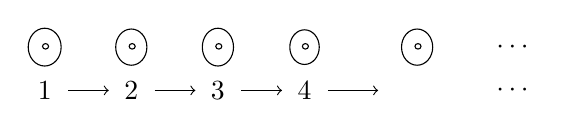
\begin{tikzpicture}[x=1.1cm,y=1cm]
\draw (0,0) ellipse (0.19 and 0.24);
\draw (0.01,0.01) circle (0.035);
\draw (1,0) ellipse (0.18 and 0.23);
\draw (1.01,0.01) circle (0.035);
\draw (2,0) ellipse (0.18 and 0.24);
\draw (2.01,0.01) circle (0.035);
\draw (3,0) ellipse (0.17 and 0.22);
\draw (3.01,0.01) circle (0.035);
\draw (4.3,0) ellipse (0.18 and 0.23);
\draw (4.31,0.01) circle (0.035);
\node at (5.4,0) {$\cdots$};
\node at (0,-0.55) {$1$};
\node at (1,-0.55) {$2$};
\node at (2,-0.55) {$3$};
\node at (3,-0.55) {$4$};
\draw[->] (0.27,-0.55) -- (0.74,-0.55);
\draw[->] (1.27,-0.55) -- (1.74,-0.55);
\draw[->] (2.27,-0.55) -- (2.74,-0.55);
\draw[->] (3.27,-0.55) -- (3.85,-0.55);
\node at (5.4,-0.55) {$\cdots$};
\end{tikzpicture}
\end{center}

Сделаем замену конф.
[зачёркнуто: \RussianUnclear{GELFAND-P001410}{structure-cancellation}{преобр. / неразборчиво}]
структуру, чтобы преобр. осталось
конформным.

% Packing problem and its two requests: (245,2330)-(1880,2950).
\underline{Задача}:

\RussianSourceFigure{GELFAND-P001410}{circle-packing}{В квадрате нарисованы четыре больших округлых контура, по два в верхнем и нижнем рядах; в промежутках и у границы имеются меньшие замкнутые кривые. Справа в сторону квадрата направлена горизонтальная стрелка с подписью «вписываем». Точные касания и принадлежность мелких пограничных дуг отдельным контурам не вполне различимы.}

\def\GelfandPackingCaption{вписываем}
\begin{center}
\begin{minipage}[t]{.46\linewidth}\vspace{0pt}\centering
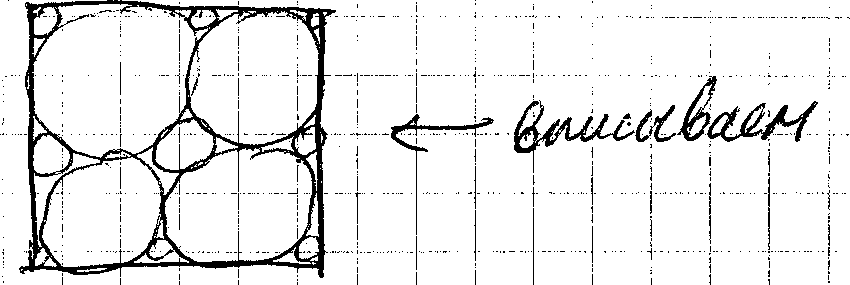
\includegraphics[width=\linewidth]{figures/gelfand-0153-p001410-circle-packing-original-r2.png}\par\smallskip
{\footnotesize Оригинал рукописного рисунка: \texttt{GELFAND-P001410}}
\end{minipage}\hfill
\begin{minipage}[t]{.50\linewidth}\vspace{0pt}\centering
{\footnotesize Частичное воссоздание видимых штрихов}\par\smallskip
\resizebox{\linewidth}{!}{% Hand-drawn contours; these coordinates do not specify exact tangencies or radii.
\begin{tikzpicture}[x=.7cm,y=.7cm]
\draw (0,0) rectangle (3,2.7);
\draw (.75,1.07) .. controls (-.05,1.16) and (-.06,2.58) .. (.7,2.64)
 .. controls (1.55,2.92) and (1.64,1.72) .. (1.43,1.37)
 .. controls (1.31,1.19) and (1.06,1.06) .. (.75,1.07);
\draw (1.5,1.43) .. controls (1.36,2.1) and (1.85,2.91) .. (2.4,2.65)
 .. controls (3.12,2.66) and (3.14,1.55) .. (2.51,1.28)
 .. controls (2.03,1.15) and (1.65,1.23) .. (1.5,1.43);
\draw (.21,.17) .. controls (.12,.76) and (.51,1.24) .. (.92,1.06)
 .. controls (1.52,.85) and (1.51,.29) .. (1.12,.08)
 .. controls (.69,-.13) and (.27,-.02) .. (.21,.17);
\draw (1.43,.31) .. controls (1.38,.73) and (1.84,1.19) .. (2.35,1.18)
 .. controls (3.14,1.34) and (3.14,.44) .. (2.79,.17)
 .. controls (2.29,-.07) and (1.56,-.07) .. (1.43,.31);
\draw (.02,2.42) .. controls (.3,2.39) and (.41,2.69) .. (.12,2.67)--cycle;
\draw (1.45,2.7) .. controls (1.66,2.32) and (1.86,2.7) .. (1.7,2.7);
\draw (2.82,2.63) .. controls (3.08,2.48) and (3.02,2.65) .. (3,2.7);
\draw (.05,.89) .. controls (.36,.75) and (.46,1.11) .. (.05,1.26)--cycle;
\draw (1.3,1.12) .. controls (1.01,.85) and (1.69,.81) .. (1.78,1.21)
 .. controls (1.65,1.44) and (1.53,1.49) .. (1.3,1.12);
\draw (2.8,1.34) .. controls (3.2,.86) and (2.71,.94) .. (2.8,1.34);
\draw (.02,.17) .. controls (.34,.04) and (.14,.3) .. (.02,.17);
\draw (1.18,.06) .. controls (1.42,.38) and (1.63,.02) .. (1.18,.06);
\draw (2.84,.04) .. controls (2.64,.24) and (3.03,.32) .. (3,.04)--cycle;
\draw[->] (4.05,1.28)--(3.43,1.23);
\node[right] at (4.05,1.28) {\GelfandPackingCaption};
\end{tikzpicture}
}
\end{minipage}
\end{center}
\noindent{\small\textit{Видимые контуры воссозданы приближённо. Точные касания, размеры окружностей и принадлежность мелких граничных дуг не установлены; количественная упаковка не задана.}}


1) Док., что остаток имеет меру $0$

2) Док., что остаток имеет хаусд. размерность $<2$.


\RussianSourceFrame{GELFAND-P001411}{46}
% Original frame: 2408 x 3448. Heading bbox (190,40,1500,195); label (2160,35,2340,140).
\underline{\underline{И.М. Гельфанд}}. \underline{Матроиды.}

% Original text bbox (205,190,2290,630); inspected in 3x crops.
В $K$-мерном пр-ве рассм. $n$ векторов;
занумеруем их и составим список: какие лин. завис., а какие — нет.
Задание этого списка — \underline{матроид}.

Какие условия на этот список?

\underline{Пример}:
[Зачёркнуто: \RussianUnclear{GELFAND-P001411}{example-cancelled}{неразборчиво}.]

% Figure bbox (305,678,590,882), enlarged 6x. Seven marked points; two solid and five outlined.
\begin{center}
\begin{minipage}[t]{.46\linewidth}\vspace{0pt}\centering
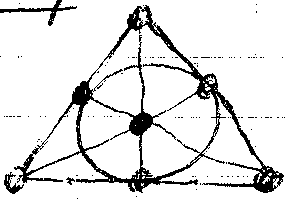
\includegraphics[width=\linewidth]{figures/gelfand-0153-p001411-fano-points-original.png}\par\smallskip
{\footnotesize Оригинал рукописного рисунка: \texttt{GELFAND-P001411}}
\end{minipage}\hfill
\begin{minipage}[t]{.50\linewidth}\vspace{0pt}\centering
{\footnotesize Частичное воссоздание видимых штрихов}\par\smallskip
\resizebox{\linewidth}{!}{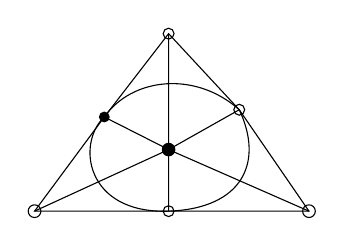
\begin{tikzpicture}[scale=1.15]
\coordinate (a) at (0,1.96);
\coordinate (b) at (-1.48,0);
\coordinate (c) at (1.55,0);
\coordinate (d) at (-0.71,1.04);
\coordinate (e) at (0.78,1.12);
\coordinate (f) at (0,0);
\coordinate (g) at (0,0.68);
\draw (a)--(d)--(b)--(f)--(c)--(e)--cycle;
\draw (a)--(g)--(f) (b)--(g)--(e) (d)--(g)--(c);
\draw (d) .. controls (-0.40,1.48) and (0.30,1.55) .. (e)
 .. controls (1.05,0.55) and (0.83,0.03) .. (f)
 .. controls (-0.92,-0.03) and (-1.02,0.75) .. (d);
\draw (a) circle (0.06) (b) circle (0.07) (c) circle (0.07)
 (e) circle (0.06) (f) circle (0.06);
\fill (d) circle (0.06) (g) circle (0.075);
\end{tikzpicture}
}
\end{minipage}
\end{center}
\noindent{\small\textit{Семь точек сохраняют две закрашенные и пять контурных отметок дипломатического рисунка. Подписи векторов не добавлены.}}


если 3 точки лежат на одной линии, то векторы
линейно зависимы.

Всё пр-во 3-мерно (нет 4-х лин. независимых)

% Original bbox (90,985,2270,1640), inspected at 3x.
(1) \underline{Задача}: 1) док., что над $\mathbb{R}$ и $\mathbb{C}$ таких векторов нет!

2) над $\mathbb{Z}/2\mathbb{Z}$ такие векторы есть.

(все ненулевые векторы у $(\mathbb{Z}/2\mathbb{Z})^3$!)

\underline{Общая} (\underline{нереш. задача}): какие матроиды реализуются
а) над $\mathbb{R}$
б) над $\mathbb{C}$.?

\underline{Решена задача}: какие матроиды реализ. над $\forall$ полем?

% Book reference bbox (190,1810,1750,2025), word enlarged 5x; glyph after Рота enlarged 7x.
\underline{В книжке Рота} \RussianUnclear{GELFAND-P001411}{book-after-rota}{э..}
[Справа: см. \RussianUnclear{GELFAND-P001411}{book-overwritten-noun}{книге?} \underline{Айгнера} (?)]
имеется 15 различных эквив. опр. матроида.

% Original bbox (75,2020,2280,2550); cancellation (1470,2315,1650,2450), enlarged 8x.
(2) \underline{Аксиоматика}.

Выделены подмн-ва, \underline{называемые базисами}

$B_1,B_2$ — 2 базиса

$y\in B_2,\ y\notin B_1\ \Rightarrow\ \exists x\in B_1;$
$(B_1\setminus x)\cup y$
[Зачёркнуто: \RussianUnclear{GELFAND-P001411}{basis-exchange-cancelled}{неразборчиво}],
$(B_2\setminus y)\cup x$ —
\newline
— базисы

\underline{Упр. из лин. алгебры}: проверить для мн-ва векторов в лин. пр-ве.

% Original bbox (50,2670,2370,3425); definition enlarged 4x and 6x.
(3) \underline{Биматроид}: рассм. матрицу; из неё опр. 2 матроида — по столбцам
и строкам

$S$ и $T$

Другое понятие: выписать все миноры $\ne0$

Биматроид: набор подмн-в с одинак. числом элементов.

(4) [Зачёркнуто: \RussianUnclear{GELFAND-P001411}{problem-four-cancelled}{неразборчиво}.]
\underline{Задача}: указать аксиомы для биматроида.


\RussianSourceFrame{GELFAND-P001412}{unlabelled}
% Original frame: 2408 x 3448; no confidently visible page label.
% Top bbox (115,55,2370,315), enlarged 3x; name (550,160,875,285), enlarged 8x.
(5) \underline{Задача}: как понятие биматроида из
[Зачёркнуто: \RussianUnclear{GELFAND-P001412}{top-cancelled}{неразборчиво}]
Гельфанда — Сергановой (УМН)
связано с \RussianUnclear{GELFAND-P001412}{knuth-name}{Кунтом}

\underline{Задача}: доказать, что

% Formula bbox (275,270,2320,425), inspected at 3x, 6x and 8x. Keep anomalous indices/sign as seen.
\begin{equation*}
\text{(6)}\quad
[x_1,\ldots,x_d][y_1,\ldots,y_d]
=\sum(-1)^{d-i}[y_1,x_2,\ldots,x_d]
[y_1,\ldots,y_{i-1},x_i,y_{i+1},\ldots,y_d]
\end{equation*}
\RussianUnclear{GELFAND-P001412}{determinant-formula-source}{индексы $y_1$, $x_i$ и знак $(-1)^{d-i}$ — по рукописи}

$[x_1,\ldots,x_d]$ — детерминант, постр. по вект.

% Original bbox (105,580,2270,810), inspected 3x.
(7) \underline{Замеч.}: если $[x_1,\ldots,x_d]$, $[y_1,\ldots,y_d]$ — базисы, то справа есть
ненулевое слагаемое — это и даёт аксиому замены
\RussianUnclear{GELFAND-P001412}{basis-axiom-reference}{(3)}

% Chain bbox (125,880,2245,1220), inspected 3x; overwritten numeral 8x.
(\RussianUnclear{GELFAND-P001412}{overwritten-eight}{8})
\underline{Задача} (нудная). Цепь сизигий по Гильберту:
\begin{equation*}
(\text{кольцо})\longmapsto
\underset{\text{— детерминанты}}{(\text{образующие})}
\longmapsto (\text{соотн. между образующими})
\end{equation*}

% Original bbox (90,1195,2210,1525), inspected 3x.
(9) (\underline{Утв.}: (6) — все соотн. между образующими)

(10) а) Написать всю цепочку!

б) Дискретизовать (комбинат. соотн. написать) всей цепочки.

% Original bbox (120,1570,2370,2150), inspected 3x; cancellation enlarged 8x.
(11) \underline{Задача}. Биматроид — список миноров $\longrightarrow$
[Зачёркнуто: \RussianUnclear{GELFAND-P001412}{problem-eleven-cancelled}{неразборчиво}]
2 матроида
(стр. и столбцы)

По 2-м матроидам строится биматроид

\RussianSourceFigure{GELFAND-P001412}{basis-grid}{Решётка из четырёх вертикальных и четырёх горизонтальных линий; слева и снизу фигурные скобки с подписями «баз…»; справа стрелка направлена влево, к решётке.}

\def\GelfandBasisLabel{баз... [?]}
\begin{center}
\begin{minipage}[t]{.46\linewidth}\vspace{0pt}\centering
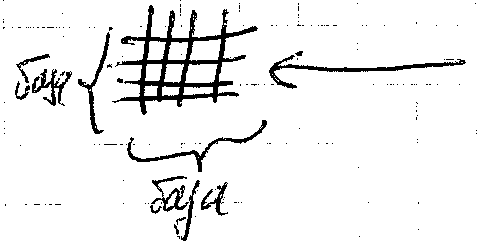
\includegraphics[width=\linewidth]{figures/gelfand-0153-p001412-basis-grid-original.png}\par\smallskip
{\footnotesize Оригинал рукописного рисунка: \texttt{GELFAND-P001412}}
\end{minipage}\hfill
\begin{minipage}[t]{.50\linewidth}\vspace{0pt}\centering
{\footnotesize Частичное воссоздание видимых штрихов}\par\smallskip
\resizebox{\linewidth}{!}{\begin{tikzpicture}[x=.75cm,y=.75cm]
\foreach \x in {0,.28,.56,.98}{\draw (\x,-.1)--(\x+.09,1.1);}
\foreach \y in {0,.15,.38,.67}{\draw (-.16,\y)--(1.26,\y+.06);}
\draw (-.3,1.05) .. controls (-.35,.8) and (-.42,.59) .. (-.56,.54)
 .. controls (-.36,.5) and (-.52,-.1) .. (-.35,-.15);
\draw (-.12,-.3) .. controls (-.31,-.71) and (.45,-.31) .. (.52,-.6)
 .. controls (.57,-.31) and (1.19,-.55) .. (1.35,-.18);
\node[left] at (-.58,.5) {\GelfandBasisLabel};
\node[below] at (.6,-.68) {\GelfandBasisLabel};
\draw[->] (2.97,.45)--(1.43,.43);
\end{tikzpicture}
}
\end{minipage}
\end{center}
\noindent{\small\textit{В обеих подписях скобок сохранено лишь начало «баз...»; окончания не установлены после просмотра при 3×, 5× и 10×. Термины базисов строк и столбцов не определяют начертание.}}


по опр. \RussianUnclear{GELFAND-P001412}{basis-construction-word}{база?}.

% Lower prose bbox (275,2130,2220,2810), inspected 3x; last adjective enlarged 6x.
Но это не обязательно.

В биматроиде больше информации.

Какова доп. информация в биматроиде?

Это важное когомологич. понятие.

\underline{Замеч.} Алгебр. топология — маленький остров в привычной
комбинат. технике.


\RussianSourceFrame{GELFAND-P001413}{unlabelled}
% Оригинал: 2408 x 3448. Координаты обзора (x0,y0,x1,y1), начало слева сверху:
% заголовок 150,65,2160,375; Керов и образующие 165,365,2230,605;
% (1) 280,600,1700,1010; (2)--(4) 80,1010,2300,1670;
% библиография 135,1700,2335,2470; конструкция и (5) 200,2530,2050,3280.
% Текстовые сомнения проверены увеличениями 3--5x, малые знаки 4--5x.
\underline{\underline{30/XI-87г.}}\qquad \underline{Сем. Гельфанда.}

\underline{И.М. Гельфанд.} Задача: найти характеры симметрической группы.

(по следам Фробениуса).

\underline{О раб.} \underline{Керова}: «\underline{Реализация предст. алгебры Геке} и т.д.»

Подсказка: это характеры симм. группы.

Алгебра Геке --- алгебра с образующими $\{e_k\}$
[над строкой: $k=1,\ldots,N-1$] и соотношениями
\begin{equation*}
\text{(1)}\quad
\left\{\begin{aligned}
e_k e_{k+1}e_k-\tau e_k&=e_{k+1}e_k e_{k+1}-\tau e_{k+1}\\
e_{k+j}e_k&=e_k e_{k+j},\quad j\geq 2;\\
e_k^2&=e_k
\end{aligned}\right.
\end{equation*}
Другие образующие
\begin{equation*}
\text{(2)}\quad \sigma_k=(q+1)e_k-1,\qquad \tau=\frac{q}{(q+1)^2}
\end{equation*}
Эта алг. обозначена $H_N(q)$.

\underline{Упражнение}: записать соотношения на $\sigma_k$.

(3) При $q=1$ (или $\tau=\frac14$) получается групповая алгебра симм. группы.

(4) \underline{Задача}: $\dim H_N(q)=N!$

[На левом поле: обведённый в круг «!».]
В работе \RussianUnclear{GELFAND-P001413}{citation-name}{Типпера / Диппера} и Джеймса

Proc. London Math. Soc.\qquad 1986, v. 52, p. 20--52

рекомендуется!!

док., что теория предст. $H_N(q)$ аналогична теории модулярных
предст. симметрической группы.

Это работает даже в комплексном случае (см. раб. Бернш.--Гельф.--Гельф.
о модулях Верма).

При этом предполагается, что $q\ne\sqrt[m]{1}$

\underline{Конструкция представлений.}

Диаграмма Юнга\quad $\lambda=(\lambda_1,\lambda_2,\ldots,\lambda_k)$

\begin{center}
(5)\qquad
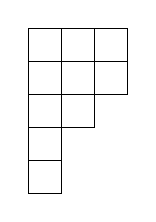
\begin{tikzpicture}[x=0.42cm,y=0.42cm]
\draw (0,0)--(3,0)--(3,-2)--(2,-2)--(2,-3)--(1,-3)--(1,-5)--(0,-5)--cycle;
\draw (1,0)--(1,-5);
\draw (2,0)--(2,-3);
\draw (0,-1)--(3,-1);
\draw (0,-2)--(3,-2);
\draw (0,-3)--(2,-3);
\draw (0,-4)--(1,-4);
\end{tikzpicture}
\qquad
$\begin{gathered}\sum\lambda_j=|\lambda|\\[8pt]\lambda_{i+1}\leq\lambda_i\end{gathered}$
\end{center}

($\lambda_i$ --- число клеток в $i$-м столбце)

Это соотв. классу сопряж. элементов.


\RussianSourceFrame{GELFAND-P001414}{52}
% Оригинал: 2408 x 3448. Координаты обзора (x0,y0,x1,y1), начало слева сверху:
% (6) 110,30,2200,410; определение и большая таблица 80,410,2250,890;
% три малые таблицы 130,940,1090,1290; (7)--(9) 100,1290,2220,2295;
% (10)--(12) 110,2330,1910,2940; (13)--(14) 65,2930,2030,3448.
% Неясные слова/штрихи просмотрены при 3--10x; новых исходных пикселей нет.
Таблица Юнга:
\begin{equation*}
\text{(6)}\quad t=\{\lambda^{(k)}\}_{k=1}^{N}
\quad\text{--- набор диаграмм, в котором}
\end{equation*}
\begin{equation*}
|\lambda^{(k)}|=k.
\end{equation*}

Обычное опред. (другое): табл. заполн. числами $1,2,\ldots,|\lambda|$, причём
\begin{equation*}
\begin{matrix}\rightarrow\\\downarrow\end{matrix}
\quad\text{по этим напр. возрастание}
\end{equation*}

% Контур большой таблицы воспроизведён без добавления внутренних линий:
% в источнике подписаны 1,2,4,7 / 3,5,8 / 6, нижняя часть длинной ножки пустая.
\begin{center}
\begin{minipage}[t]{.46\linewidth}\vspace{0pt}\centering
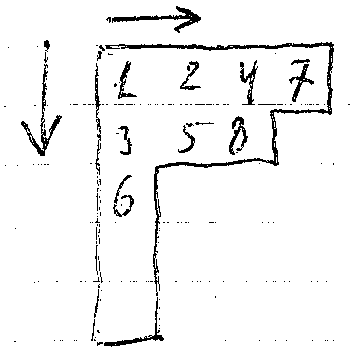
\includegraphics[width=\linewidth]{figures/gelfand-0153-p001414-young-tableau-original.png}\par\smallskip
{\footnotesize Оригинал рукописного рисунка: \texttt{GELFAND-P001414}}
\end{minipage}\hfill
\begin{minipage}[t]{.50\linewidth}\vspace{0pt}\centering
{\footnotesize Частичное воссоздание видимых штрихов}\par\smallskip
\resizebox{\linewidth}{!}{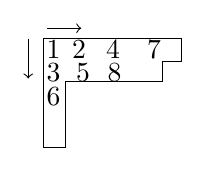
\begin{tikzpicture}[x=0.44cm,y=0.44cm]
\draw (0,0)--(4,0)--(4,-0.65)--(3.45,-0.65)--(3.45,-1.25)--(0.65,-1.25)--(0.65,-3.15)--(0,-3.15)--cycle;
\node at (0.30,-0.33) {$1$};
\node at (1.04,-0.33) {$2$};
\node at (2.02,-0.33) {$4$};
\node at (3.20,-0.33) {$7$};
\node at (0.30,-0.97) {$3$};
\node at (1.15,-0.97) {$5$};
\node at (2.06,-0.97) {$8$};
\node at (0.30,-1.66) {$6$};
\draw[->] (0.12,0.30)--(1.10,0.30);
\draw[->] (-0.43,0.0)--(-0.43,-1.15);
\end{tikzpicture}
}
\end{minipage}
\end{center}
\noindent{\small\textit{Сохранены неровный контур и восемь видимых чисел. Пустая длинная ножка не заполнена; внутренняя сетка клеток не добавлена.}}


В (6) они должны возрастать

\begin{center}
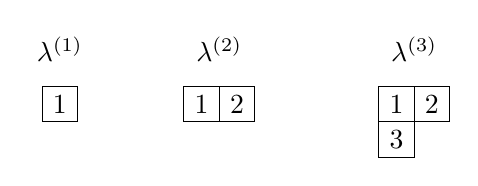
\begin{tikzpicture}[x=0.45cm,y=0.45cm]
\node at (0.5,1.05) {$\lambda^{(1)}$};
\draw (0,0) rectangle (1,-1);
\node at (0.5,-0.5) {$1$};
\node at (5,1.05) {$\lambda^{(2)}$};
\draw (4,0) rectangle (6,-1);
\draw (5,0)--(5,-1);
\node at (4.5,-0.5) {$1$};
\node at (5.5,-0.5) {$2$};
\node at (10.5,1.05) {$\lambda^{(3)}$};
\draw (9.5,0)--(11.5,0)--(11.5,-1)--(10.5,-1)--(10.5,-2)--(9.5,-2)--cycle;
\draw (10.5,0)--(10.5,-1);
\draw (9.5,-1)--(10.5,-1);
\node at (10,-0.5) {$1$};
\node at (11,-0.5) {$2$};
\node at (10,-1.5) {$3$};
\end{tikzpicture}
\end{center}

\begin{equation*}
\text{(7)}\quad r_k(t)=(i_{k+1}-j_{k+1})-(i_k-j_k)
\end{equation*}
точка $k$ имеет координаты $(i_k,j_k)$

Для диаграммы:
\begin{equation*}
\text{(8)}\quad h(\lambda)=r_\lambda+1
\end{equation*}
\begin{equation*}
\text{(9)}\quad r_\lambda=\max_{t\in T(\lambda)}\max_{1\leq k<N}|r_k(t)|,
\end{equation*}
где $T(\lambda)$ --- мн-во таблиц, построенных по диаграмме $\lambda$, т.е.
имеющих форму $\lambda$.

Пусть $s=(\mu^{(k)})_{k=1}^{N}$,\quad $t=(\lambda^{(k)})_{k=1}^{N}$.

(10) \underline{Опр.}\quad $s\underset{n}{\approx}t$, если $\lambda^{(k)}=\mu^{(k)}$, $k\ne n$

\underline{Утверждение.}

(11) [Зачёркнуто: \RussianUnclear{GELFAND-P001414}{eq11-cancelled-word}{если?};
над строкой вставлено: Пусть]
$r_n(t)=\pm1$; тогда $s\underset{n}{\approx}t\Rightarrow s=t$;

(12) Пусть $|r_n(t)|>1$; тогда $\exists!\ s:\quad s\underset{n}{\approx}t$, $s\ne t$.

\begin{equation*}
\text{(13)}\quad S_\lambda^{(k)}=\Vert S_{s,t}^{(k)}(\tau)\Vert_{s,t\in T(\lambda)}
\quad\text{--- матрица};
\end{equation*}
[После индекса у матрицы, ниже строки:
\RussianUnclear{GELFAND-P001414}{eq13-terminal-mark}{неразборчивый знак; $q$ / исправленная запятая}.]

\begin{equation*}
\text{(14)}\quad
S_{s,t}^{(k)}(\tau)=\bigl(W_{r_k(s)}(\tau)\ W_{r_k(t)}(\tau)\bigr)^{1/2}
\quad\text{при }s\underset{k}{\approx}t
\end{equation*}
[После первого множителя, ниже строки:
\RussianUnclear{GELFAND-P001414}{eq14-blotted-mark}{замазанный или зачёркнутый знак}.]

[Зачёркнуто: \RussianUnclear{GELFAND-P001414}{eq14-cancelled-condition}{при $s\underset{k}{\approx}t$?}]
и $S_{s,t}^{(k)}(\tau)=0$ в противном случае.

